\section{Improving JVT using Attention}\hfill

The JVT model used by ATLAS is used to classify jets as HS or PU. However, in high pileup conditions JVT algorithm will need to be improved. Here we benchmark the JVT kNN algorithm~\cite{ATLAS-CONF-2014-018} against AttnJVT.

%\subsection{Jet Features}\hfill
%Each jet has 6 features which includes the kinematic 4-vector of each jet, $p_T, \eta, \phi, m$ as well as track dependent features $corrJVF, Rp_T$ which were first proposed by ATLAS~\cite{ATLAS-CONF-2014-018}. First, corrJVF can be understood as the fraction of the jet's momentum coming from hard scatter particles originating from the primary vertex with respect to the total momentum coming from all other vertices. However, it has been shown that this variable has a dependence on $\left<\mu\right>$, so to correct for this behavior the contribution from pileup vertices are normalized by the number of pileup particles in the event and a free parameter, k. This parameter has been shown to best remove dependence on $\left<\mu\right>$ at k=0.01~\cite{ATLAS-CONF-2014-018}.
%\begin{equation}
%    corrJVF = \frac{\sum\limits_k p_T^{trk_k}(PV_0)}{\sum\limits_l p_T^{trk_l}(PV_0)+\frac{\sum\limits_{n\geq1}\sum\limits_l p_T^{trk_l}(PV_n)}{(k \cdot n^{PU}_{trk})}}
%\end{equation}

%\begin{figure}[h!]
%\centering
%\begin{subfigure}{.45\textwidth}
%  \centering
%  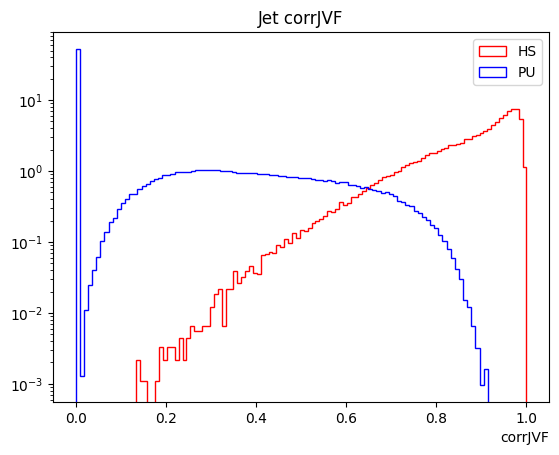
\includegraphics[width=0.9\linewidth]{corrJVF}
%  \caption{}
%  \label{fig:sub1}
%\end{subfigure}
%\begin{subfigure}{.45\textwidth}
%  \centering
%  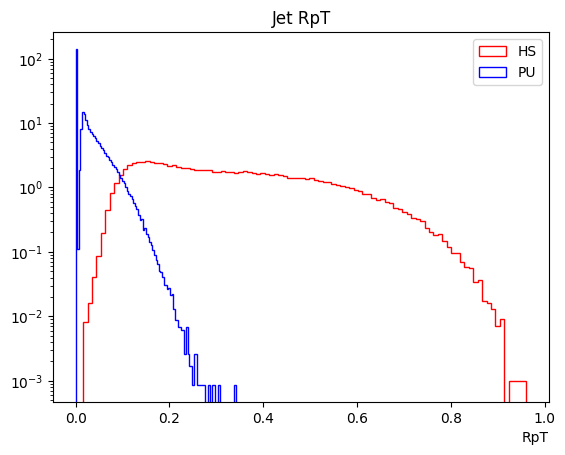
\includegraphics[width=0.9\linewidth]{RpT}
%  \caption{}
% \label{fig:sub2}
%end{subfigure}
%\caption{Figure (a) The distribution of corrJVF for Hard Scatter jets and PileUp jets.. Figure (b) The %istribution of $R_{pT}$ for Hard Scatter jets and PileUp jets.}
%label{fig:test}
%\end{figure}

%Second, $R_{pT}$ can be understood as the fraction of the jet's momentum originating from hard scatter primary vertex.
%\begin{equation}
%    R_{pT} = \frac{\sum_kp_T^{trk_k}(PV_0)}{p_T^{jet}}
%\end{equation}

%These features have unique distributions for HS and PU jets. HS jets tend to have higher corrJVF and RpT than pileup jets as shown in figure [*]. \\

%\begin{figure}[h!]
%\centering
%\begin{subfigure}{.25\textwidth}
%  \centering
%  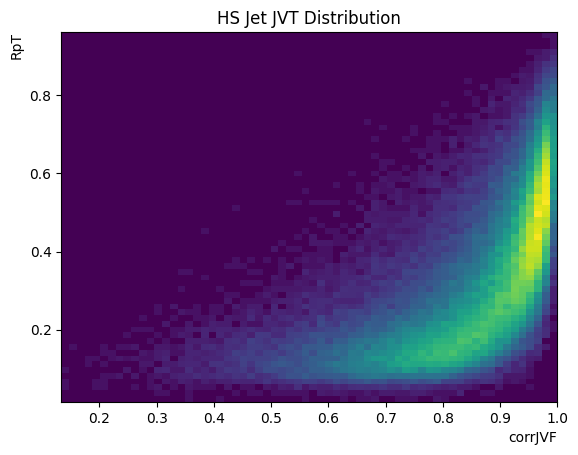
\includegraphics[width=0.9\linewidth]{HS}
%  \caption{}
%  \label{fig:sub1}
%\end{subfigure}%
%\begin{subfigure}{.25\textwidth}
%  \centering
%  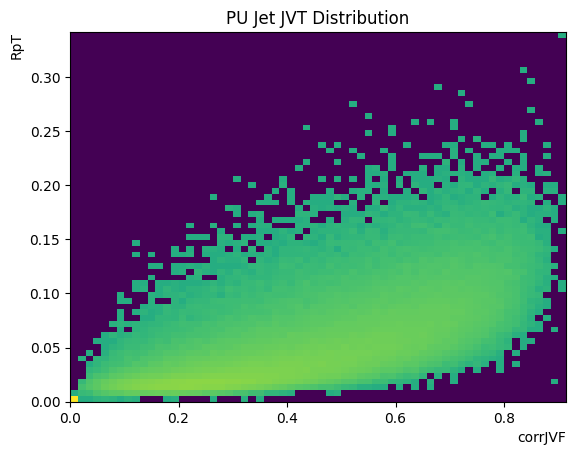
\includegraphics[width=0.9\linewidth]{PU}
%  \caption{}
%  \label{fig:sub2}
%\end{subfigure}
%\caption{Distribution of jets in the $R_{pT}$-corrJVF plane for (a) HS and (b) PU jets.}
%\label{fig:test}
%\end{figure}

\subsection{Jet Labels}\hfill

To fairly benchmark JVT and AttnJVT, a binary label was constructed by cutting on the squared sum of the constituent particle's $p_T$.

\begin{equation}
    PU_{fr} = \frac{\sum\limits_{PU} p_T^{2}}{\sum\limits_{HS} p_T^{2} + \sum\limits_{PU} p_T^{2}}
\end{equation}

An arbitrary cut is imposed on this distribution to convert the continuous distribution into a binary distribution. This cut allows for a consistent and fair benchmark against existing models. In this study, HS jets have $PU_{fr}<0.7$ and PU jets have $PU_{fr}>0.7$.

\begin{figure}[h]
\centering
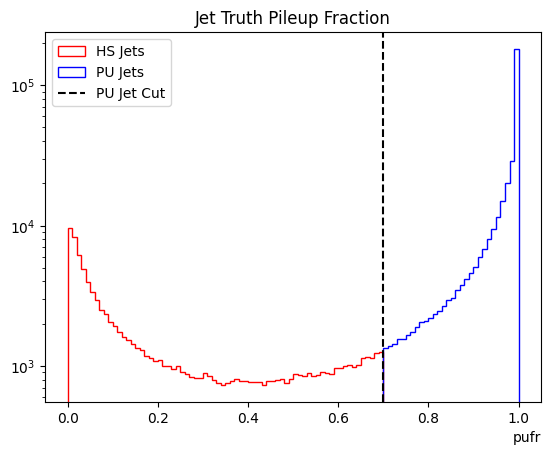
\includegraphics[width=0.3\textwidth]{PU_Jet_Cut}
\caption{An arbitrary cut on the continuous $PU_{fr}$ to recover binary labels.}
\end{figure}

\subsection{Classical JVT Architecture}\hfill

The Jet Vertex Tagger, JVT, was orignally proposed by ATLAS~\cite{ATLAS-CONF-2014-018}. The model uses $R_{pT}$ and corrJVF as input and constructs a likelihood between zero and one which represents the probability in which the jet originated from hard scatter. The JVT model is based on a k-Nearest Neighbor, kNN, algorithm which uses a Euclidean metric in the $R_{pT}$-corrJVF plane and is fit using k=100.

\begin{figure}[h!]
\centering
\begin{subfigure}{.3\textwidth}
  \centering
  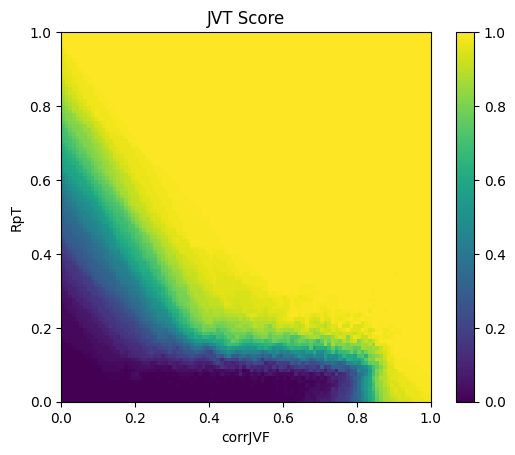
\includegraphics[width=0.9\linewidth]{JVT_2d}
  \caption{}
  \label{fig:sub1}
\end{subfigure}%
\begin{subfigure}{.3\textwidth}
  \centering
  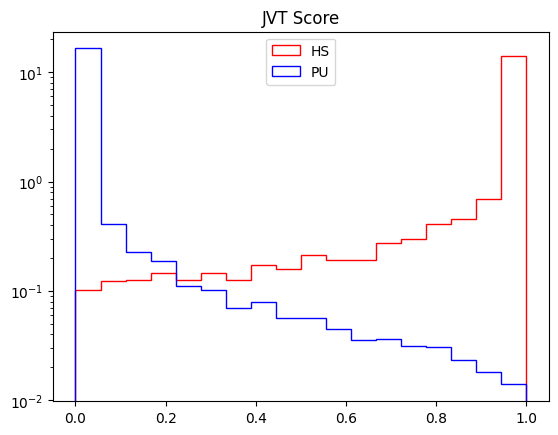
\includegraphics[width=1\linewidth]{JVT_1d}
  \caption{}
  \label{fig:sub2}
\end{subfigure}
\caption{Figure (a) shows JVT liklihood in the $R_{pT}$-corrJVF plane. Figure (b) shows the JVT liklihood for HS and PU jets.}
\label{fig:test}
\end{figure}

\subsection{AttnJVT Architecure}\hfill

To perform a fair benchmark, the orignal JVT model was recreated and performance was evaluated between the original model and the attention model on the same dataset. The input to the model is a unordered set of jets from an event. Each event has a variable number of jets, N, so the input tensor will be of shape $\mathbb{J} \in \mathbb{R}^{N,F}$ where F is the six input features described in section 2.1. The input jets are fed through an initializer, $\phi$, to transform them into the embedding space with dimension D:

\begin{equation}
\phi(\mathbb{J}) \rightarrow \mathbb{E} \in \mathbb{R}^{N,D} 
\end{equation}

The embedded jets are then passed through a multi-head attention layer to update their representations in the context of an entire event. First the embeddings $\mathbb{E}$ are passed through a multi-head attention layer using self attention to generate the context tensor $\mathbb{C}$:

\begin{equation}
\mathbb{C} = MHA(\mathbb{E},\mathbb{E},\mathbb{E})
\end{equation}

Then the context tensor, $\mathbb{C} \in \mathbb{R}^{N,D}$, is concatenated with the original embedding to update the original representation of each jet, $\mathbb{E} = \mathbb{E}+\mathbb{C}$. Lastly, the jet embedding is passed through a final classifier, $\Psi$, to perform binary classification:

\begin{equation}
\Psi(\mathbb{E}) \rightarrow \vec{y} \in \{0,1\}
\end{equation}

The model is trained using the Binary Cross Entropy loss function.

\begin{figure}[h!]
\centering
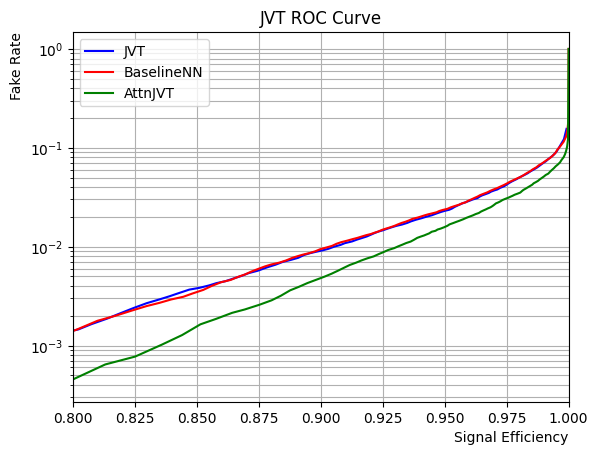
\includegraphics[width=0.5\textwidth]{AttnJVT}
\caption{Using a MHA layer, the jets have access to the context of the entire event which allows the model to capture correlations between HS jets. This effect reduces the fake rate of the model.}
\label{fig:test}
\end{figure}

We benchmarked JVT against AttnJVT to show that we can reduce the fake-rate when we use a Multihead Attention layer which gives jets event context. This event-wide context allows the model to learn correlations between HS jets.